\section{24. März 2015}

\question{Franck-Condon-Prinzip und Intensität der Übergänge}
\label{q:51}

Siehe \aqref{25}.

\question{Diskutiere die Elektronenkonfiguration von \ch{N2}.}
\label{q:52}

\[\ch{N_2} : (1\sigma_g)^2 ~ (1\sigma_u^*)^2 ~ (2\sigma_g)^2 ~ (2\sigma_u^*)^2 ~ (1\pi_u)^4 ~ (3\sigma_g)^2\]
14 Elektronen werden auf die $\pi$- und $\sigma$-Bindungen aufgeteilt. Achtung: Die Reihenfolge der $1\pi$- und der $3\sigma$-Orbitale kann variieren. Die unterschiedliche Reihenfolge dieser Orbitale kommt durch eine Mischung der s- und p-Atomorbitale zustande: Eine solche kann vorkommen, wenn der energetische Unterschied zwischen dem 2s- und dem 2p-Orbital der Atome klein genug ist (N$_2$ bildet genau die Grenze, bis zu der die Bildung dieser Mischung möglich ist). Dadurch wird zwar das $2\sigma_g$-Orbital stärker bindend, das $3\sigma_g$ wird jedoch schwächer bindend. Dadurch ist das $1\pi_u$-Orbital energetisch günstiger als das $3\sigma_g$ (\autoref{fig:q52}). Ist der (energetische) Abstand zwischen den s- und p-Atomorbitalen groß genug, so kann die Mischung der Orbitale vernachlässigt werden.

\begin{figure}[H]
    \centering
    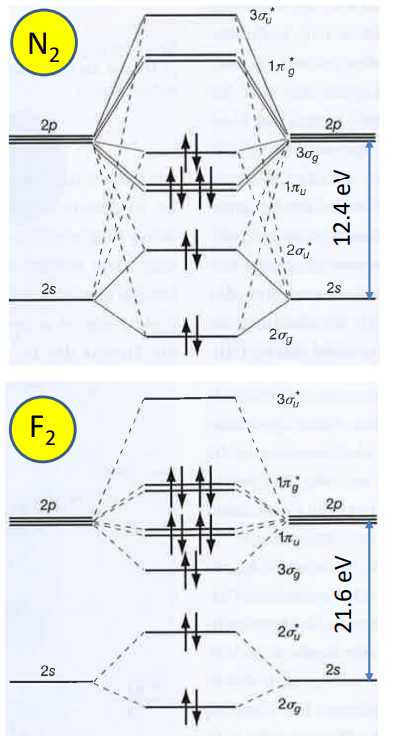
\includegraphics[width=.4\textwidth]{resources/24-03-2015/N2-F2.png}
    \caption{Elektronische Struktur von N$_2$ und F$_2$.}
    \label{fig:q52}
\end{figure}


\question{Diskutiere die Van der Waals Wechselwirkung und das Lennard-Jones Potential.}
\label{q:53}

Befindet sich ein neutrales Atom in einem elektrischen Feld $\vb{E}$, so induziert das Feld ein Dipolmoment $\vb{p_{ind}}$. Umgekehrt kann durch ein bestehendes Dipolmoment $\vb{p_A}$ aber auch ein elektrisches Feld entstehen -- aus der Multipolentwicklung des elektrischen Feldes einer Ladungsverteilung ergibt sich für den Dipolanteil:
\begin{equation*}
    \vb{E}(\vb{p_A}) = \frac{1}{4\pi\varepsilon_0 R^3} (3 p_A \vb{\hat{R}} \cos{\theta_A} - \vb{p_A})
\end{equation*}
Ein neutrales Atom mit kugelsymmetrischer Elektronenhülle weist über die Zeit gemittelt aufgrund der Bewegung der Elektronen kein Dipolmoment auf -- trotzdem hat ein solches Atom immer ein momentanes Dipolmoment. Dadurch entsteht ein elektrisches Feld, welches in einem anderen neutralen Atom ein Dipolmoment induzieren kann. Diese Wechselwirkung neutraler Atome ist die van-der-Waals-Wechselwirkung. Sie ist relativ schwach im Vergleich zu einer Ionenbindung und vor allem kurzreichweitig. Für das van-der-Waals-Potential gilt:
\begin{equation}
    E_{pot}(R) = -\frac{C}{R^6}
\end{equation}
Um das Potential noch besser zu beschreiben wird das empirisch ermittelte Lennard-Jones-Potential verwendet, das zusätzlich zum anziehenden Term des van-der-Waals-Potenzials noch einen abstoßenden Term berücksichtigt:
\begin{equation}
    E_{pot}(R) = \frac{a}{R^{12}} - \frac{b}{R^6}
\end{equation}
Dabei sind $a$ und $b$ Anpassungsparameter, die so gewählt werden, dass das Potenzial dem experimentell bestimmten Potenzial in möglichst guter Näherung entspricht. Durch die Kombination von anziehendem und abstoßendem Term entsteht ein Minimum des Potenzials beim Bindungsabstand mit $E_B = E_{pot}(R_e) = \frac{b^2}{4a}$.


\question{Konzept des Bravaisgitters und der Wigner-Seitz-Zelle.}
\label{q:54}

Ein Bravaisgitter ist ein rein mathematisches Gitter, welches die Periodizität eines Kristallgitters beschreiben soll. An die einzelnen Gitterpunkte des periodischen Bravaisgitters können im Prinzip beliebig komplizierte Kombinationen von Atomen oder Molekülen gesetzt werden, die dann als Basis bezeichnet werden. Das Bravaisgitter beschreibt also nur die Periodizität, die Basis beschreibt die konkrete Struktur des Kristalls. Wichtig: Die Anordnung und Orientierung der Punkte im Bravaisgitter müssen identisch sein, egal von welchem Punkt man es betrachtet.

In einem solchen Gitter lassen sich unterschiedliche Arten von Einheitszellen definieren. Die Wigner-Seitz-Zelle lässt sich konstruieren, indem man:
\begin{itemize}
    \item ein Atom mit allen seinen Nachbarn verbindet
    \item Die Mittelsenkrechte auf alle Verbindungslinien konstruiert (in 3D entspricht das einer Ebene)
    \item Die von diesen Flächen eingeschlossene Fläche entspricht dann der Wigner-Seitz-Einheitszelle
\end{itemize}
Anmerkung: Konstruiert man die Wigner-Seitz-Einheitszelle im reziproken Gitter, so entspricht diese der 1. Brillouin-Zone.

\question{Diskutiere den Unterschied zwischen der akustischen und optischen Phononendispersionsrelation bzw. longitudinaler/transversaler, akustischer und optischer Phononen.}
\label{q:55}

Betrachtet man eine eindimensionale Kette aus zwei abwechselnd aufeinander folgenden Atomen $M_1$ und $M_2$, welche durch eine Hook'sche Feder verbunden sind, und löst die zugehörige Bewegungsgleichung, so ergibt sich daraus eine quadratische Gleichung für die Frequenz $\omega$. Die beiden Lösungen dieser Gleichung sind der optische und der akustische Ast, wobei der optische Ast nur dann auftritt, wenn die Kette tatsächlich aus einer zweiatomigen Basis besteht. Bei einer einatomigen Basis gibt es nur den akustischen Ast. Der optische Ast weist außerdem eine höhere Frequenz auf. Durch die unterschiedliche räumliche Orientierung der Schwingung lassen sich der akustische und der optische Ast weiters in transversale und longitudinale Äste einteilen. Bei $s$ Atomen pro Einheitszelle ergeben sich immer $3$ akustische Freiheitsgrade und $3s-3$ optische Freiheitsgrade (also insgesamt $3s$ Schwingungsäste).
% eventuell noch ausbaufähig

\question{Diskutiere das statische Verhalten des freien Elektronengases.}
\label{q:56}

Eine der Annahmen des klassischen Drude-Modells zur Beschreibung der Elektronen als freies Elektronengas schließt Kollisionen zwischen Elektronen aus und beschränkt sich somit nur auf Stöße zwischen Elektronen und Atomrümpfen. Letztere werden dabei als statisch betrachtet. Im Modell werden zusammengefasst die folgenden Annahmen getroffen:

\begin{enumerate}
    \item ideales Elektronengas: Keine WW zwischen den Elektronen
    \item Elektronen kollidieren nur mit Atomrümpfen, nicht untereinander
    \item Die Geschwindigkeit der Elektronen nach einem Stoß korreliert mit der Temperatur und ist somit vom herrschenden thermodynamischen Gleichgewicht abhängig
    \item Die mittlere freie Weglänge liegt in der Größenordnung der Atomabstände
\end{enumerate}

\question{Diskutiere die Einstein- und Debye-Näherung der Wärmekapazität.}
\label{q:57}

Siehe auch \aqref{7} und \aqref{40}.

Grundprämissen Wärmekapazität klassisches Modell: \( c_v = \pdv{U}{T} \big\rvert_V \) und \( U = \frac{f}{2} k_B T = 3 k_B T \). Damit ergibt sich: \( c_{v, m} = 3 k_B N_A = 3R \) (Dulong-Petit-Gesetz).

\vspace{.2cm}
\hrule
\vspace{.2cm}

Grundprämissen quantenmechanisches Modell: System aus N harmonischen Oszillatoren mit \( E_n = \hbar \omega \left(n + \frac{1}{2}\right) \): 

\[ \langle U \rangle = 3N \frac{\sum_{n=0}^\infty E_n e^{-\frac{E_n}{k_B T}}}{\sum_{n=0}^\infty e^{-\frac{E_n}{k_B T}}} \] 

\[ [\dots] \Rightarrow \langle U \rangle = 3N\hbar\omega_k\left(\frac{1}{2}+\langle n_k\rangle \right) = 3N\hbar\omega_k\left(\frac{1}{2}+ \frac{1}{e^{\frac{\hbar\omega_k}{k_BT}}-1} \right) \] 

oder als Integral mit der Zustandsdichte:

\[ \langle U \rangle = \displaystyle\int_{1. BZ} 3N\hbar\omega_k\left(\frac{1}{2}+\langle n_k\rangle \right) Z(k) d^3k = \displaystyle\int_{\omega_{min}}^{\omega_{max}} 3N\hbar\omega_k\left(\frac{1}{2}+\langle n_k\rangle \right) D(\omega) d\omega\]

\vspace{.2cm}
\hrule
\vspace{.2cm}

Einstein-Modell: Alle Atome schwingen mit der gleichen Frequenz $\omega_E$, d.h. $D(\omega) = \delta(\omega-\omega_E)$.

\[\Rightarrow c_v^E  = \pdv{U}{T} \bigg\rvert_V  = \left\{ \begin{array}{ll}
    e^{-\frac{\Theta_E}{T}} & T \ll \Theta_E \\
    3 N_A k_B  & T \gg \Theta_E \\
    \end{array} \right. 
\]

Dabei beschreibt $\Theta_E = \frac{\hbar \omega_E}{k_B}$ die Einstein-Temperatur.
Einstein-Modell funktioniert gut bei hoher Dichte an optischen Photonen, berücksichtigt aber keine akustischen Phononen und versagt bei tiefen Temperaturen.

\vspace{.2cm}
\hrule
\vspace{.2cm}

Debye-Modell: 3 Annahmen

\begin{enumerate}
    \item Lineare Dispersion $\omega_i = v_i k$
    \item Isotrope Schallgeschwindigkeit $v_1 = v_2 = v_3 = v_s$
    \item Erste Brillouinzone hat die Form einer Kugel mit Radius $k_D$, sodass die Anzahl der Schwingungsmoden innerhalb der Kugel gleich der Anzahl der Atome im Kristall ist.     
\end{enumerate}

Für ein kontinuierliches gilt: $D(\omega) = \frac{V}{(2\pi)^3} \left( \frac{1}{v_L^3} + \frac{2}{v_T^3}\right) \omega^2$ und es ergibt sich mit den 3 Annahmen:

\[ D(\omega) \left\{ \begin{array}{ll}
    \frac{3V}{(2\pi)^3} \frac{\omega^2}{v_s^3} & \omega \ll \omega_D \\
    0  & \omega \gg \omega_D \\
    \end{array} \right.
\] 

sowie für die Wärmekapazität:

\[ c_v^D \cong \left\{ \begin{array}{ll}
    T^3 & T \ll \Theta_D \\
    3N_Ak_B  & T \gg \Theta_D \\
    \end{array} \right.
\] 
Dabei beschreibt $\Theta_D = \frac{\hbar \omega_D}{k_B}$ die Debye-Temperatur.
Durch die Berücksichtigung der akustischen Phononen funktioniert das Debye-Modell bei tiefen Temperaturen besser. Dafür werden optische Phononen nicht berücksichtigt, weshalb Effekte nahe der Brillouinzonengrenze nicht richtig beschrieben werden. Im Limit hoher Temperaturen ergibt sich jedoch wieder das Dulong-Petit-Gesetz.

\vspace{.2cm}
\hrule
\vspace{.2cm}
 
\question{Diskutiere den Beitrag der Elektronen zur Wärmekapazität.}
\label{q:58}

Das Drude-Modell (klassisches Modell, siehe \aqref{56}) versagt im Hinblick auf den Beitrag der Elektronen zu der Wärmekapazität: Es ergibt zu hohe Werte für die Wärmekapazität, die den Dulong-Petit-Wert ($3N_Ak_B$) übersteigen. Besser beschrieben wird der Beitrag durch das (quantenmechanische) Sommerfeld-Modell. Dieses beschreibt die Elektronen als nichtwechselwirkende Teilchen in einem unendlichen Potenzialtopf. Die Zustandsdichte $D(E)$ wird hier zusätzlich mit der Fermi-Dirac-Statistik $f_{FD} (E, T)$ modifiziert, um die fermionischen Eigenschaften der Elektronen zu berücksichtigen.

\[ U(T) = \displaystyle \int_0^\infty E f_{FD}(E,T) D(E) dE \]

Die resultierende Zustandsdichte ist in \autoref{fig:q58} dargestellt. Für die Wärmekapazität des freien Elektronengases ergibt sich dann \( c_v = \frac{1}{2} \pi^2 nk_B \frac{T}{T_F} = \gamma T\). 

\begin{figure}[H]
    \centering
    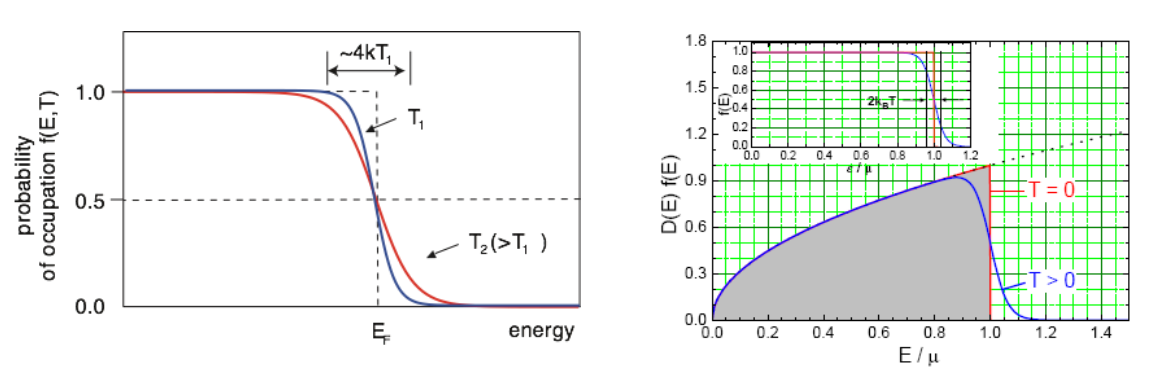
\includegraphics[width=\textwidth]{resources/24-03-2015/D(E)f(E).png}
    \caption{Fermifunktion und Zustandsdichte der Energie.}
    \label{fig:q58}
\end{figure}

\question{Was besagt das Bloch-Theorem bzw. die Bloch-Funktion?}
\label{q:59}

Bei einem periodischen Potential (z.B. der Überlagerung der Coulomb-Potentiale in einem Kristallgitter) können die Lösungen der Schrödinger Gleichung als Linearkombinationen von Basisfunktionen der Form

\[ \Psi_k(\vb{r}) = u_k(\vb{r}) e^{i\vb{k}\vb{r}}\]

mit \( u_k(\vb{r}) = u_k(\vb{r} + \vb{R}) \), d.h. mit einer Basis aus einer periodischen sogenannten Bloch-Funktion $u_k$ und einer Exponentialfunktion, dargestellt werden. Zeigen lässt sich dies, indem sowohl $\Psi$ als auch $U$ als komplexe Fourier-Reihe dargestellt werden. Die $u_k$ haben die Form

\[ u_k(\vb{R}) = \displaystyle \sum_{\vb{G}} c_{\vb{k}-\vb{G}}  e^{-i \vb{G} \vb{r}} \]

Die Fourier-Koeffizienten $c_{\vb{k}-\vb{G}}$ können aus folgendem Gleichungssystem berechnet werden, das auch als Hauptgleichung bezeichnet wird:

\[ \left( \frac{\hbar^2 k^2}{2m} - E \right) c_k + \displaystyle \sum_G U_G c_{k-G} = 0 \]

Dabei sind die $U_G$ die Koeffizienten der Fourier-Darstellung des Potenzials. Das Bloch-Theorem ist nützlich zur Berechnung der elektronischen Bandstruktur $E_n(k)$ eines Kristalls. 

\question{Welche Arten von Dia- und Paramagnetismus kennen Sie?}
\label{q:60}

Siehe \aqref{32}.

\newpage